\documentclass[12pt]{article}
\usepackage{verbatim}
\usepackage[dvips]{epsfig}
\usepackage{color}
\usepackage{url}
\usepackage[colorlinks=true]{hyperref}
\usepackage[margin=0.5in]{geometry}
\usepackage{sidecap}

\begin{document}

\noindent Program Director/Principal Investigator (Last, First, Middle): Bower, James M.

\subsection*{DRAFT 5.0}

\subsection*{Title: Multi-scale modeling synaptic plasticity in cerebellar cortex: Implications for aging\\P.I.: James M. Bower}

\subsection*{Abstract}

This highly collaborative multi-scale modeling project interweaves a number of different scientific and technical objectives each of which, on their own, will advance their fields. Because the project is based in GENESIS, an existing and widely used modeling system, the effort will also provide a paradigm shifting technical capability for multi-scale modeling with application to a wide range of biological problems. The core premise of this project is that models, and especially those that reflect the actual structure of biological data, will increasingly become essential tools to organize experimental data, direct new experimental designs and eventually interpret the functional significance of the data generated. They will also become a mechanism for coordination and communication of scientific results and efforts. In this larger context, the core scientific objective of this project is to construct the first ever biologically realistic multi-scale model of the cerebellum from molecular to systems levels. The cerebellum is ideally suited for this kind of effort because the basic organization of its circuitry has been known for more than 100 years, and as a result most hypothesis regarding cerebellar function are linked to the structure's anatomy and physiology. In fact, this modeling effort will be organized to test and contrast two such hypotheses which represent very different views of the functional role of molecular layer synaptic plasticity in cerebellar function, a question that has been at the center of theoretical and experimental cerebellar investigations for more than 50 years. Once developed this model will also be used to establish the cerebellum as a model system to assess effects of aging and aging interventions on the central nervous system. To fulfill these ambitious objectives this project brings together a unique and diverse set of collaborators with both modeling and experimental experience at multiple different levels of scale as well as an advisory group of specialists in brain related aging research.

%PHS 398/2590 (Rev. 06/09)
\newpage

{\center \subsection*{SPECIFIC AIMS}}
The overall objective of this proposal is to accomplish four interrelated and mutually supporting specific aims:

\paragraph{Aim 1: Develop the technical capability to inter-link heterogeneous biologically realistic models across multiple levels of spatio-temporal scale within the new G-3 architecture.} One central design objective of the GENESIS system is to provide a common modeling platform to support the development of realistic biological models requiring different levels of scale. This has allowed GENESIS models to be built at all scales from molecular through large scale networks and systems. The original GENESIS architecture, however, did not readily support the necessary interaction amongst heterogeneous model components to efficiently connect them into a unified model and the incorporation of new components and simulator functionality was difficult and time consuming. Over the last several years, the core structure of the GENESIS simulator has been fundamentally redesigned to speed the process of adding new modeling capacity at different levels of scale.
%Additionally, the new software architecture of GENESIS explicitly supports interaction amongst heterogeneous model components.
Accordingly, the primary technical objective of this project is to develop the capacity to inter-link biologically realistic models across different levels of scale as opposed to each model at a single model of scale.

\paragraph{Aim 2: To construct a multi-scale model of cerebellar cortex to explore the functional significance of molecular layer synaptic plasticity.} The primary scientific objective of this project is to construct the first multi-scale biologically realistic model of cerebellar cortical networks, extending from molecular to system levels. The cerebellum is particularly well suited to this effort because its structural organization has been understood for more than 100 years and there is abundantly available experimental data on that structure. The specific focus of the effort will be on the functional role of molecular layer synaptic plasticity, which has been extensively studied ever since Marr and Albus independently proposed a novel parallel fiber synaptic modification mechanism in the late 1960s (Marr, 1969; Albus, 1971). The modeling effort will be organized around comparing and contrasting the original Marr/Albus hypothesis which assumes that parallel fiber inputs directly affect the output spiking of Purkinje cells, with a more recent hypothesis that parallel fibers provide a modulatory function and do not directly drive Purkinje cell output (Bower, 2011). In the Marr/Abus formulation, the plastic properties of parallel fiber synapses determine which parallel fibers drive Purkinje cell output, while, in the alternative formulation, parallel fiber plasticity instead provides a general metabolic regulation of the relative strength of parallel fiber inputs with respect to molecular layer inhibition. Linking biological realistic simulations together at multiple levels of scale will allow us to formally test the implications of each hypothesis at different levels of scale.

\paragraph{Aim 3: To apply the multi-scale modeling effort to quantify possible effects of the cerebellum on aging.} The P.I. has recently become a member of the Barshop Institute for Aging and Longevity Studies at the University of Texas Health Science Center in San Antonio. As a member of this Institute, he is charged with brining modeling techniques, specifically with respect to the cerebellum to bear on aging studies. In fact, the cerebellum represents a unique structure with which to assess the neuronal effects of normal aging, as well as the neuronal consequences of aging interventions. The cerebellum undergoes greater volume atrophy and cell loss than any other known brain region and behaviors like motor performance, traditionally ascribed to the cerebellum are directly affected by aging. Further, specific cerebellar cellular mechanisms, like parallel fiber LTD, are known to also be affected by the normal aging process. While we recognize that linking experimentally measured changes in neuronal properties to behavioral measures is an ambitious task, the model to be developed here will begin the process of establishing a more solid foundation for such investigations.

\paragraph{Aim 4: Disseminate both the models developed and the tools for multi-scale modeling to the computational neuroscience community as a whole.} From the outset the GENESIS project has placed a significant emphasis on the development of supporting materials for the broader dissemination and use of models both as research and educational tools. Therefore, an important objective of this project is to introduce and support tools that will allow computational neuroscience access to multi-scale modeling technology.

{\centering \subsection*{RESEARCH STRATEGY}}

{\centering \subsection*{A. Significance}}

\noindent This highly collaborative multi-scale modeling project interweaves a number of different scientific and technical objectives each of which, on their own, will advance their fields. Because the project is based in GENESIS, this effort will also provide access to paradigm shifting technical tools for multi-scale modeling with anticipated application to a wide range of biological problems. Figure 1 illustrates graphically the partnership plan linking each of the participants in this project which represent a strong set of collaborators with diverse and overlapping expertise in both multi-scale modeling and experimental investigations.\\

\subsubsection*{A.1 Providing a new framework to organize and consider cerebellar experimental data.}

It is a core principle of the P.I.'s laboratory and of the laboratories of the collaborators, that models will increasingly become essential tools to organize experimental data, direct new experimental designs, and eventually interpret the functional significance of the data generated. Further, it is a core principle of our efforts that the models that are most useful in performing these functions will be those that are built in close relationship to the existing experimental data (Bower, 1992; Bower, 2005; Bower and Beeman, 2007). Accordingly, the overarching aim of this project is to develop a multi-scale model of cerebellar cortical circuitry based on a new set of multi-scale modeling tools to be constructed within the GENESIS simulation system (Bower and Beeman, 2007). Through the GENESIS system, these new multi-scale modeling tools as well as the models themselves will be fully accessible, providing the basis for ongoing dialog and collaboration. In fact, this collaboration came together because members of the team have already been engaged in such a scientific model-based dialog using the Purkinje cell model that has become one of the first `community models' in computational neuroscience (Bower 2011a). That model, which is also at the core of this project, was originally based on a passive Purkinje cell model published by Rapp, Segev, and Yarom almost 15 years ago (Rapp et al.,1994), to which, after Importing the model into GENESIS, the P.I. together with his then postdoctoral fellow, Erik De Schutter introducing active conductances (De Schutter and Bower, 1994a;b;c). Since 1994, this single Purkinje cell model has formed the basis for a series of ongoing studies within the Bower laboratory (Jaeger et al., 1997; Jaeger and Bower, 1999; Santamaria et al., 2002; 2007; Santamaria and Bower, 2005; Cornelis and Bower, 2007), and has also served as the basis for ongoing collaborations and studies in and between the laboratories of the P.I.s former students and postdocs (Steuber and De Schutter, 2001; Salinas et a., 2006, 2007; Steuber et al., 2007; Shin et al., 2007; De Schutter and Steuber, 2009: Coop et al., 2010; Anwar et al., 2010; Hendrickson et al., 2011a;b). Importantly, the same model has also been used by other laboratories not directly related to the Bower lab (Miyasho et al., 2001; Coop and Reeke, 2001; Chono et al., 2003; Traub et al., 2008; De Sousa et al., 2009; Luthman et al., 2011). Of significance to the current proposal, this model has also served as the basis for the construction of a model at the network level of scale (Luthman et al., 2009; Maex \& Steuber, 2009; Santamaria et al., 2009). With this history as an existence proof, this new project will enhance the Purkinje cell model at the subcellular level, and test an improved model at the network level with open access policies, producing the first multi-scale community model in computational neuroscience.\\

\noindent [Figure 1 in here somewhere]

\subsubsection*{A.2 Specific scientific context: What is the role of molecular-layer synaptic plasticity in cerebellar function?}

It is also a core tenant of this collaborating team that even technical progress in science is best made when efforts are focused on a particular scientific question. In this case, the question of the role of molecular layer plasticity in cerebellar function has been at the forefront of discussions and debates regarding the cerebellum for almost half a century, since David Marr and Jim Albus independently speculated that changes in molecular layer synaptic strengths supported the function of the cerebellum as a pattern classifier that could learn to generate an appropriate output in response to arbitrary inputs (Marr 1969; Albus, 1971). Inspired by the contrast between the hundreds of thousands of synapses converging on each Purkinje cell from the mossy fiber $\neq$ granule cell pathway, and the climbing fiber pathway where each Purkinje cell is innervated (in the adult) by only one axon, it was specifically proposed that the strengths of parallel fiber synapses were changed by coincident climbing fiber activation. When Masao Ito and his colleagues reported that parallel fibers underwent long term depression (LTD) in response to coincident climbing fiber activation (Ito et al., 1982), it set the stage for what has been a very large number of studies of cerebellar synaptic plasticity. In fact, a recent Pubmed search with the key words `cerebellum' and `plasticity' reveals more than 100 peer reviewed scientific papers published since the start of 2011 alone, with almost 75\% focused at the level of molecular mechanisms.\\

\noindent While the question of cerebellar plasticity has received a very large amount of experimental attention, it remains quite unclear what role plasticity plays in cerebellar function (contrast: De Zeeuw, 2011 with Vogt and Canepari, 2010 for example).\\

\noindent Accordingly, the central scientific objective of this effort will be to construct a multi-scale model to link experimental data at multiple levels of scale in order to quantitatively explore the possible roles of molecular layer plasticity in cerebellar function. To provide further focus to the project, we will initially use the model to contrast the original Marr/Albus proposal with a second, more recent hypothesis that proposes a very different functional role for parallel fiber synaptic plasticity. In the case of Marr/Albus and most other theories of the function of cerebellar cortex, it is assumed that parallel fiber activity is directly responsible for driving the output of the cerebellar Purkinje cell (Marr 1969; Albus 1971). In contrast, recent experimental and modeling work suggests instead that parallel fiber inputs do not directly drive Purkinje cell output but instead are `modulatory' in nature (Jaeger and Bower 1999). Specifically it has been proposed that parallel fiber excitatory inputs, working in concert with inhibitory inputs from molecular layer interneurons, generate a form of voltage clamp control over local regions of the Purkinje cell dendrite. This controlled voltage, in turn, influences the large calcium and related potassium conductances in the dendrites which, in turn, influence the firing of the Purkinje cell soma. Further details on this hypothesis can be obtained from a recently published review (Bower, 2011). However, the important point for the current project is that if this new hypothesis is correct, then activity dependent changes in molecular layer synapses may play a significant role in regulating the balance between excitatory and inhibitory synaptic inputs rather than providing an explicit learning mechanism (De Schutter, 1995; De Schutter, 1997). As discussed in more detail below, the other important point is that these two theories for the role of synaptic plasticity make very different functional predictions at multiple different levels of scale.

\subsubsection*{A.3 The cerebellum as a model system for studying aging.}

While the question of the role of synaptic plasticity in cerebellar function is at the heart of many contemporary cerebellar theories (see Ito, 2006 for review), circumstances also provide an opportunity to explicitly link the question of cerebellar learning to a larger and significant issue in human health: the role of the cerebellum in aging. Specifically in September of 2011, the P.I. joined the Barshop Institute for Longevity and Aging Studies at the University of Texas Health Science Center in San Antonio with two specific objectives: first to introduce computation tools, including multi-scale modeling, to the larger institute; and second to further develop the cerebellum as a model system for studying the aging process as well as treatments that affect aging (such as caloric restriction and drugs like rapamycin). The multi-scale model to be constructed here will be central to both objectives. In fact, there are several clear links between the cerebellum and aging. First, it has been known for almost 100 years (Ellis 1919) that cerebellar volume is significantly reduced during aging and it is now known that the anterior lobe in humans can undergo up to a 15\% volume reduction by age 70 with a 45\% loss in the number of Purkinje cells (Andersen et al., 2003). This reduction in volume and cell number is larger than any so far reported for other mammalian brain structures. At the same time, functions traditionally associated with the cerebellum including balance, grip, and over all motor related behaviors are all affected in aging populations and associated with aging related diseases (for reviews see: Dominguez and Magro, 2009; Christou 2011; Vonsattel et al., 2011). Further, recent reports suggest aged mice are reduced in their performance of classical operant eye blink conditioning, a task some believe is also dependent on normal cerebellar function (Woodruff-Pak et al., 2010). Our own recent studies in normal humans and those with cerebellar deficits suggest that the cerebellum may influence the ability to detect pitch or to localize sound in space (Petacchi et al., 2005; 2011; Parsons et al., 2009;), both deficits known to occur in aging populations as well (for review see Huang and Tang 2010).\\

\noindent While there would appear to be an explicit link between the cerebellum and behavior changes in aging, as with the cerebellar research as a whole, links between behavioral measures and actual biophysical and molecular aging effects will remain largely circumstantial and correlational in the absence of a model linking together different levels of experimental scale. For example, in the study of eye blink conditioning in aging mice, the authors also report a reduced capacity for parallel fiber LTD (Woodruff-Pak et al., 2010). Is that correlation causal, or could the reduced parallel fiber synaptic plasticity disrupt the homeostatic regulation of synaptic input, resulting in premature cell death of Purkinje cells? Further, does the reduced performance of the mice in the eye blink conditioning task reflect a decreased capacity for cerebellar learning, or a decreased ability of the mice to detect the pitch associated with the conditioned stimulus (c.f. Parsons et al., 2009; Petacchi et al., 2005; 2011). While we recognize that any effort to link cellular to behavioral changes in aging or any behavioral measure is complex and difficult, ultimately we would claim that any such linkage is very likely to depend on the existence of a multi-scale model linking observations at different levels of scale. In later sections we describe specific questions that will be asked of the model generated by this project as a first step in that direction.

{\centering \subsection*{B. Innovation}}

At the heart of the innovation represented by this project is the construction of the first ever biologically realistic multi-scale model in computational neuroscience. While some existing computational cerebellar models mix and match biological components at different levels of scale (for example, synaptic learning rules in large scale abstract systems models: c.f. Ohyama et al., 2010 and related models), this is the first effort to link fully detailed realistic models across multiple levels of scale. Accordingly, this project will embed models of biochemical and molecular mechanisms at the level of individual synapses (the work of collaborators Blackwell and Kubota) to models of Ca$^{2+}$ diffusion and buffering in spine heads (Blackwell, Santamaria, Kubota) and local regions of the dendrite (Kubota, Santamaria, Bower), to models of synaptic and ion channel interactions at the cellular level (Santamaria, Bower and Jaeger), to patterns of activity determined by network connectivity and the pattern of afferent inputs (Bower, Jaeger and Steuber).\\

\subsubsection*{B.1 The GENERAL NEURAL SIMULATION SYSTEM (GENESIS)}

The\marginpar{here need both technical and CS framework} GENESIS
simulation system is at the core of the necessary technical innovation
for this project. As such this project extends the long history of
innovation in the GENESIS project (Bower and Beeman, 2006; 2007;
Beeman, 2011). For example, GENESIS provided the first graphical
modeling interface (Uhley et al., 1990; Bower and Hale 1991), the
first computational neuroscience website (1994), and also the first
use of virtual reality techniques for visualizing results (Leigh et
al., 1995). The GENESIS group also established the first standards to
judge the speed and reliability of neural simulators (Bhalla et al.,
1992), and the first tools to quantify parameter searches and modeling
results (Eichler-West, 1996; Baldi et al., 1998; Vanier and Bower,
1999). GENESIS was also one of the first computational modeling
systems to be run on parallel computers (Nelson et al., 1989; De
Schutter and Bower, 1992). Moreover, the GENESIS development group has
also been deeply involved in efforts to provide interoperability
between neural simulators (Beeman and Bower, 2004; Cannon, et al.,
2007), beginning with the Modelers Workspace project
(www.modelersworkspace.org) which drafted and promoted the first
markup language for realistic neural modeling (Goddard, et al., 2001).
These early efforts motivated the formation of the NeuroML project
(Crook, et al., 2007), which has subsequently fostered the development
of community modeling tools such as neuroConstruct (Gleeson, et. al.,
2007) and will also be a core component of this project. The GENESIS
group also pioneered the use of modeling databases as sources of
biological data (Hucka, et al., 2002), spawning a major middleware
software project, now called The System's Biology Workbench (Hucka, et
al., 2001:http://www.sbw-sbml.org/), which has played an important
role in the development of multi-scale models in molecular and
cellular biology. GENESIS also served as the basis for the first set
of simulation-based tutorials for education in neuroscience through
the publication of The Book of GENESIS (Bower and Beeman, 1998) and
has so far been used for instruction in neuroscience and computational
neuroscience in more than 60 universities around the world (Beeman,
2011). %This project will add another stage of innovation to GENESIS.

\begin{SCfigure}
%\centering
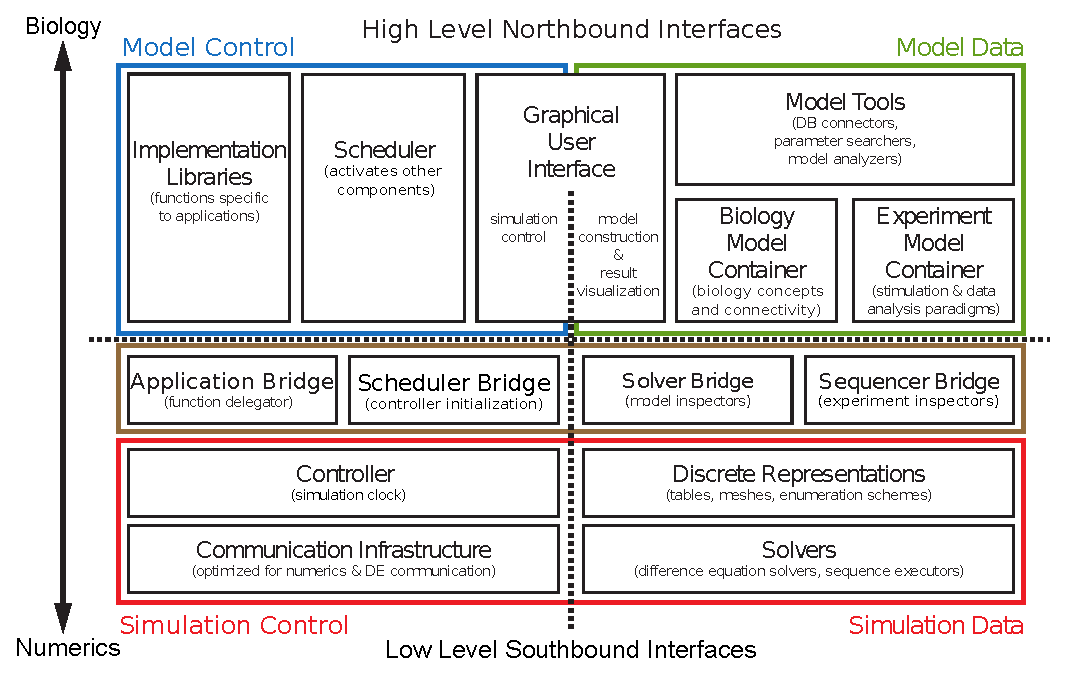
\includegraphics[scale=0.56]{figures/cbi-architecture-expanded.eps}
\caption{\footnotesize {\bf Detailed view of the Computational Biology Initiative
    federated software architecture.}  This figure shows a graphical
  representation of the core structure of G-3. In sharp contrast to
  previous versions of GENESIS and other neuronal simulation
  platforms, the design of G-3 is fundamentally modular, separating
  different functional components of the simulator into their own
  modules. Importantly, G-3 separates model descriptions from the
  mathematical representations used in actual model simulation. This
  simplifies the implementation of new solvers and other
  simulation time software components. The communication infrastructure
  connects different solvers simulating the same model and can
  `upscale' or `downscale' numerical data as needed. For additional
  detail see Cornelis et al. 2011a;b.  }
\label{fig:cbi-architecture-expanded}
\end{SCfigure}
%\hspace{0.5cm}
%\begin{minipage}[b]{0.5\linewidth}
%\centering
%\includegraphics[scale=1]{filename2}
%\caption{default}
%\label{fig:figure2}
%\end{minipage}
%\begin{figure}[ht]
%\begin{center}
%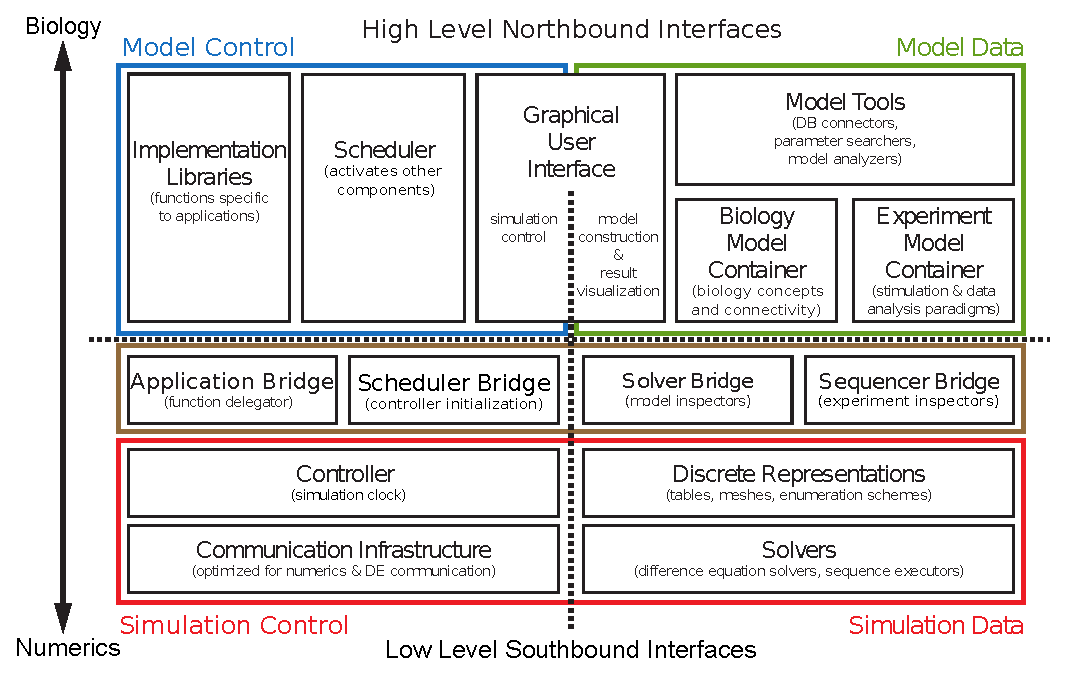
\includegraphics[width=5in]{figures/cbi-architecture-expanded.eps}
%\end{center}



Many neuroscience simulators, including G-2, allow simulation at
subcellular, cellular, or network scales, but are also restricted
to each level of scale.  The monolithic nature of these simulators makes it
almost impossible to extend their functionalities
beyond the particular levels they support.

In contrast, the new modular structure and the communication module of
G-3 are key to its extensible multi-scale capabilities (described in
more detail below).

Importantly, because of its modular structure, G-3 allows in principle
the incorporation of both traditional multi-scale techniques such as:
multi-grid method, fast multi-pole method, domain decomposition and
adaptive mesh refinement and wavelet based methods; and more recent
multi-scale techniques such as quasi-continuum method, heterogeneous
multi-scale modeling and adaptive model refinement.  The distinction
between these two methods is that the traditional multi-scale
techniques capture the macroscale behaviour of a system by simulation
of microscale models, while the more recent techniques capture system
behaviour by coupling macroscale and microscale models.  This
distinction puts them in different modules of the G-3 simulator
architecture.

The modular structure allows for rapid incorporation of new
solvers at a specific scale (see below for an example) while,
in compliance with the G-3 software architecture and this facilitated extensibility, scale-separation between solvers is maintained through the implementation of different types of run-time
interfaces between concurrent solvers.
%the
%communication module allows implementation of different types of run-time
%interfaces between concurrent solvers, thereby effectively maintaining
%the scale-separation between these solvers, keeping them fundamentally
%compliant with the modular structure of G-3 and keeping them
%extensible to meet new user needs. 
At its essence, these two new
features of G-3 transform multi-scale modeling in
neuroscience from today's implementation of individual models at specific levels of scale to a systematic
technique where a comprehensive software foundation enables simulation across different levels.


\subsubsection*{B.2 Multi-scale modeling.}

Of direct relevance to the innovation represented by this grant,
GENESIS was the first and remains the only simulation system
specifically designed from the outset to support modeling at multiple
levels of biological scale (Bower and Beeman, 2006; 2007; Brette et
al., 2007). Reflecting this history, a recent survey of 324
peer-reviewed GENESIS publications (not involving the P.I. as an
author) revealing that 50\% involved networklevel models with most
describing large networks up to 10,000 neurons: 40\% were based on
models of single neurons; and 10\% were constructed to explore the
interaction of subcellular molecular components.  This project will
add significantly to the tools already available for subcellular level
modeling (Bhalla and Iyengar, 1999; Bhalla, 2002; Sivakumaran, et al.,
2003) while also adding additional capacity to build large scale
network models. 

The Discrete Event System is a software of G-3 with the specific aim
to support large scale network modeling by storing action potentials
as discrete events that are delivered at post-synaptic target sites at
appropriate times.

With its translation function between the discrete event domain and
continuous time, the DES system interfaces between mathematical
solvers and event queues, and links across scales the simulation
objects that run at their own specific scale.

Critical in the implementation of this scale-link is the existence of
a single model-container that integrates the model across scales
during its construction phase.  The addressing algorithm of the
model-container provides the capability to obtain the addresses of
solved variables residing in different solvers independent of their
scale\marginpar{this seems written upside down}.

When combined the single model-container and the addressing algorithm
allow to instantiate efficient communication components embedding any
type of numerical scheme or algorithm required to run a simulation of
an aspect of the integrated model.  As described in the next section,
the most innovative as well as challenging technical aspect of this
project\marginpar{way to many occurences of 'this project'} involves
the development of tools that cross link and embed finer scale models
in cellular and network level simulations.


\subsubsection*{B.3 The new ``Scale-link'' functionality.}

Over\marginpar{expand computer science background, describe innovation
  as a paradigm shift, see cbi-multiscale} the last 5 years with
support from the National Institute of Neurological Disorders and
Stroke at NIH (R01 NS049288-05), the GENESIS development team has
completely redesigned and modernized the core structure of GENESIS
producing GENESIS version 3.0 or G-3. These changes are briefly
described in the introduction of the ``Approach'' section of this
grant, however, the important point with respect to innovation is that
the new structure of G-3 provides a new and unique capacity for
federated and modular software development in support of multi-scale
modeling. Furthermore, G-3s structure also supports the direct real
time interaction, or embedding of models at different levels of scale.
As described in more detail below, this is accomplished through
specific software modules that create intermediary representation of
variables present at multiple scales as described in more detail in
subsequent sections. It is important to note that while the structure
of G-3 supports this kind of functionality, there is no
support\marginpar{relate to CBI: there is only support for expansion
  of the scope of the upper layer, but not for expansion of the scope
  of the lower layer} the development of the tools necessary for
multi-scale modeling in the current NIH grant. Instead that grant is
focused on reorganizing and modernizing the core of the simulator, on
user support, tutorial generation, and the necessary extensive
documentation of the new system. Of course, the NINDS grant also does
not support the specific scientific objective of constructing a
multi-scale cerebellar model.  Accordingly, although synergistic,
there is no overlap between these two grants. This new project will,
however, add a capability to G-3 anticipated to considerably expand
its value to the computational neuroscience community.

{\centering \subsection*{C. Approach}}

\subsubsection*{C.1 GENESIS as the basis for our approach.}

Before considering our specific approach to each of the Specific Aims
of this project, it is first necessary to describe the way in which
G-3 specifically supports this multi-scale modeling effort. As
described in more detail in Cornelis, et al, (2011a; b), a key
component of G-3, which is also central to its use in multi-scale
modeling, is a redesign around two workflows, one for the user and a
second for developers. The user workflow now makes explicit the
linkage between modeling and experimental results with support, for
example, experimental protocols like RTXI (Cornelis and Coop,
2010)\marginpar{this seems unnecessary}.  Because streamlining the
process of adapting and extending GENESIS was also a key objective of
the redesign, G-3 fundamentally modular structure now supports the
independence but also the interoperability of different software
components of the overall system. Of direct relevance to the current
project, these changes: (1) reduce the complexity of software modules
when compared to a more traditional monolithic system (prior versions
of GENESIS and NEURON for example), (2) simplify documentation of
modules in terms of inputs and outputs, (3) more easily incorporate
new simulation modules like Chemsis and CDS for example (see below),
and (4) simplify development and testing of modules as stand-alone
components. Overall, the effect is to provide a much clearer
delineation of the scope for new module development\marginpar{unclear
  how the workflows do this, explain the workflows as complementary to
  the CBI architecture}, including the addition of modules operating
at different levels of modeling scale.  The G3 architecture is also
'federated' as it extends the modular approach associated with the
development of single applications to the functional integration of
otherwise independent applications. As such it provides a single
collaboration framework for modeling and software tool development. As
described in the next section these changes have already been used to
rapidly incorporate new molecular scale modeling capacity into the
overall system. They will be essential to add additional modeling
capacity at other levels of scale, as well as the software components
necessary for models at different levels of scale to interact.

\subsubsection*{C.2 Specific Aim 1: Develop the Technical Capability
  to scale-link biologically realistic simulations at multiple levels
  of scale using the new G-3 architecture.}

Having described the overall new features of G-3 that make this
project possible, in this section we will describe our specific
approach to adding the capacity to construct detailed subcellular
molecular/biochemical, and biophysical models, as well as large scale
network of systems level models\marginpar{communication framework
  description, embed in computer science background}. Given
limitations in space, we will not describe G-3s implementation of
single compartmental neurons, or small-scale neuronal networks.
GENESIS implementation for these models has been extensively described
elsewhere (Bower and Beeman 2006; 2007). In addition, in this section
we will briefly describe the technical approach to linking models at
different levels of scale.  With respect to time lines and outcomes,
development of the technical capability to support these different
modeling scales and their interaction will be continuous over the
entire 5 years of the grant and will be coordinated by the Bower
laboratory in partnership with the other collaborators. Individual
time lines and expected outcomes will be described in section C.3 for
specific components of the multi-scale cerebellar model which will be
used as a test case for all technical implementations.

\paragraph{C.2.1. Sub-cellular level modeling.} Key to the success of this project will be the expansion of tools for constructing sub-cellular level models. Accordingly, as a test of the new multi-scale modeling capacity of G-3 we began working in May of 2011 with Dr. Avrama Blackwell (now a collaborator on this grant) to incorporate the core functionality of Chemesis (Blackwell 2000, Blackwell and Kotleski 2002) into the structure into G-3. ``Chemesis'' which supports the modeling of biochemical reactions, second messengers, and calcium dynamics (Blackwell, 2000) was originally added on to GENESIS version 2.0 by adding user-contributed library over multiple years. In contrast, the core features of Chemesis-3 were added to G-3 in under 3 months with ``Chemesis-3'' now running almost three times faster than in GENESIS-2. This rapid and successful incorporation was a result of several explicit features of G-3, including: 1) the modular separation of the development of the core of new solvers from that of other software components, allowing full focus on the mathematical aspects of the solver and their implementation, and better optimization; 2) the G-3 Developer package facilitated integration of the Chemesis-3 solver into the build system of G-3 enabling immediate regression tests; 3) easy extension of the configuration of the model-container to establish new declarative model tokens and parameters recognized by the existing Chemesis-3 solvers; 4) easy construction of an interface between the model-container application programmers interface (API) and the core of the Chemesis3 solver and finally 5) the specific development of a software module that interfaces the new solver with the existing linear cable solver. In addition to the further implementation of Chemesis-3, we will use the same G-3 functionality to add biochemical kinetic modeling system being developed under MOOSE (Bhalla and Iyengar, 1999; Bhalla, 2002; Sivakumaran, et al., 2003; Ray and Bhala, 2008) to this project. \\

\noindent With\marginpar{link with computer science} respect to the
scientific objective of this project and thus Specific Aim \#2, these
new sub-cellular modeling capabilities will allow us to model pre and
postsynaptic molecular mechanisms involved in synaptic plasticity.
Further, because each of these sub-cellular modeling components are an
integrated part of a single `model' container (see Cornelis 2011a),
the existing and new G-3 solvers can be integrated to simulate
different aspects of the same model. This 'scale-linking'
functionality of G-3 instantiates dedicated run-time software
components that contain intermediary representations of solved
variables that can pass both ``upscale'' and ``downscale'' values to
simulations at different levels of scale.  Technically, in the case of
Chemesis-3 and the linear cable solver, for example, these modules
calculate weighted space-time averages.

\paragraph{C.2.2 Biophysical models of calcium diffusion and buffering.} In support and in relationship to the new molecular kinetic modeling features that will be added to G-3, this project will also work to incorporate two types of 3-D Monte Carlo-based techniques for modeling reaction/diffusion kinetics. Specifically, Dr. Avrama Blackwell will work with the G-3 development team to implement NeuroRD (Oliveira et al., 2010), a computationally efficient approximate Monte Carlo approach to modeling reaction-diffusion systems. In addition, the G-3 development team will work with Dr. Yoshi Kubota to incorporate ``CDS'' (Cellular Dynamics Simulator: http://nba.uth.tmc.edu/cds/) a precise particle-based Monte Carlo simulator specifically supporting the modeling of Ca$^{2+}$ binding and diffusion dynamics within biochemical networks (Byrne et al. 2010; Kubota and Waxham 2011). CDS is based on the event-driven first passage time algorithm (Byrne et al. 2010) and is designed to serve as a flexible platform for multi-scale hybrid algorithms. For this reason, the CDS algorithm can be directly combined with any deterministic ODE/PDE (Reaction-Diffusion Equation) solvers (e.g., V-Cell used in Hernjak et al. 2005) including those already included in G-3. High-resolution cellular morphology including that of dendritic spines can be directly transported to CDS allowing electro-diffusion to be simulated by both deterministic (as in Lopreore et al. 2008) as well as particle-based 3-D stochastic methods. The CDS research team will work closely with NeuroRD and G-3 developing team to establish a series of hybrid algorithms applicable to several different model scales. This will allow us to compare different simulation algorithms for Ca$^{2+}$ binding diffusion, voltage clamp, and biochemical network within the same platform and will help derive and validate simplified macroscopic (biochemical) synaptic rules relevant to the objectives of Specific Aim 2.\\

\noindent From a technical point of view, the incorporation of
simulations modules that specifically involve spatial dimensions is,
in principle, much more difficult than the integration of biochemical
kinetic models. In fact the accurate representation of space and time
for multi-scale simulations is an open research area and will be one
of the core technical challenges in this project. However, the
explicit provision of software modules for the intermediary
representation of solved variables will allow us to compare and
evaluate different methods of scale-linking, for instance by comparing
different resolutions of a fixed grid with adaptive grid intermediary
representations (Bernabeul et al., 2009). In effect, this will allow
us to use multi-scale G-3 models as a framework to compare different
technical strategies\marginpar{single change in a configuration file
  of the user workflow instantiates the same simulation with different
  software components, producing alternative performance and other
  results of the same simulated model}.

\paragraph{C.2.3 Single compartmental neuronal models.} Since GENESIS was first launched it has been used extensively to construct compartmental models at the single cell level. This project, in fact, is based on a Purkinje cell model which has been extensively tested and used in multiple laboratories over the last 20 years (De Schutter and Bower, 1994a;b;c; Jaeger et al., 1997; Jaeger and Bower, 1999; Steuber and De Schutter, 2001; Miyasho et al., 2001; Coop and Reeke, 2001; Santamaria et al., 2002; 2007; Chono et al., 2003; Santamaria and Bower, 2005; Cornelis and Bower, 2007; Maux and Deschutter, 2007; Steuber et al., 2007; Shin et al., 2007; Traub et al., 2008; De Sousa et al., 2009; De Schutter and Steuber, 2009: Luthman et al., 2009; 2011; Maex \& Steuber, 2009; Santamaria et al., 2009; Coop et al., 2010; Anwar et al., 2010; Hendrickson et al., 2011a;b). This model, like most compartmental models, is based on the actual anatomical geometry of a mammalian Purkinje cell (Rapp et al., 1994) to which have been added the major synaptic and voltage related conductances in the form of equivalent circuit representations of Hodgkin-Huxley dynamics (Santamaria and Bower, 2008). As part of this project, and as described below, the conductances in this model will be updated and enhanced with newly available experimental data.

\paragraph{C.2.4 Large--scale network level modeling.} As already described GENESIS has been used since the outset to build network level models of neuronal circuits. In fact, the original structure of GENESIS itself was based on a network simulation of olfactory cortex (Beeman, 2011). As part of this project, we will expand the technical capability for G-3 to support the construction of very large scale network and system models based on more abstracted neuronal components. In support of this function, the G-3 model-container applies specific algorithms to instantiate systems level connectivity models and convert them to mathematical representations, relieving the mathematical solvers from the pressure typical for rich heterogeneous model structures. At the same time, the intermediate simulation system modules already described as the mechanism used to link Chemesis-3 and the linear cable solver, will also be used to share values and functions between larger scale network simulations and lower scale models. The long term (Nelson et al., 1989; De Schutter and Bower, 1992) and intrinsic support for use of parallel computing resources within the GENESIS system will also be critical to the ability to run these large scale models (Cornelis 2011a; b) with the large scale simulations being carried out on Linux clusters of 100-500 CPU cores. 

\subsubsection*{C.3 Specific Aim 2A: Constructing a multi-scale model of cerebellar cortex to explore the functional significance of molecular layer synaptic plasticity}

For the sake of overall clarity, we have chosen to divide our approach to Specific Aim 2 into the implementation of the multi-scale cerebellar model, and then the specific use of the model to test conflicting hypothesis regarding the role of synaptic plasticity in cerebellar function. Each specific objective described here is followed by both an expected time line as well as the specific partnership plan associated with the implementation of each component of the model.

\paragraph{C.3.1 Biophysical modeling of single compartments of the Purkinje cell dendrite.} One can argue that all computational properties of neurons are determined by electrochemical interactions at sub-cellular levels. Therefore, the development of models of synaptic plasticity for example, will first depend on the construction of a biophysically accurate model of small regions of the Purkinje cell dendrite (Cornelis, 2007). To do so we will use recently obtained serial electronmicroscopic reconstructions of 5 $\neq$ 10 micrometer lengths of Purkinje cell dendrite which include the explicit locations of excitatory and inhibitory synaptic inputs (Lu et al, 2009). This data includes complete reconstructions of the locations and shapes of dendritic spines on 40 segments. As expected, parallel fiber (granule cell) synapses are located on the spines while inhibitory inputs from molecular layer interneurons are located directly on the dendritic shafts. Once these segments are represented in G-3, we will include Ca$^{2+}$ diffusion and buffering mechanisms using the newly incorporated ``CDS'' modules. Using the model we will be able to study the effects of synaptic activity and dendritic structure on Ca$^{2+}$ diffusion and buffering mechanisms. Importantly, using the multi-scale modeling capabilities of G-3, during simulations each of these high-resolution segments of the dendrite will be embedded in a larger full Purkinje cell compartmental model. In this way, local changes in Ca$^{2+}$ concentration as well as voltage will be influenced by and in turn influence neighboring compartments. Based on our previous experimental and computational work (Santamaria et al., 2006, 2011) we would predict little effect of dendritic structure on the diffusion rates of Ca$^{2+}$; however, anomalous diffusion of buffers could arise in longer time windows (Santamaria, 2011).\\

\noindent The expected timeline for construction of this model is 1 year and will be carried out as a collaboration between the Bower, Santamaria, and Kubota laboratories. The model once constructed, will be tested against confocal calcium diffusion data available from Santamaria (Santamaria,et al., 2006).

\paragraph{C.3.2 Modeling the detailed biochemical networks underlying multiple forms of plasticity.} Having established a high resolution dendritic segment model within the larger Purkinje cell multi-compartmental model, we will next further extend the resolution of the overall multi-scale model by including pre- and post synaptic molecular mechanisms using the `Chemesis' tools and either NeuroRD (Oliveira et al., 2010) or CDS depending on the requirements of the simulation. The goal of this study is to better understand how molecular level pathway changes will remain localized to single spines or spread to neighboring areas in a detailed Purkinje cell dendritic morphology reconstructed from EM data (Santamaria et al., 2006). Understanding the spatial spread of specific pathway interactions is important to determine the presence or absence of synaptic specificity of synaptic plasticity rules based on distinct biochemical pathway interactions. Specifically, we will implement the LTD specific signaling pathways activated by metabotropic glutamate receptors (Kotaleski et al. 2002), leading to calcium release and activation of protein kinase C (Ito et al., 1982), as well as the NO $\neq$ PKG pathways, known to be involved in non-specific (Wang et al., 2000; Reynolds \&Hartell, 2000; Hartell, 1996) LTD. We also will model molecules of the PI3 kinase/AKT/mTOR pathway, which are activated by tyrosine kinase receptors, and are involved in aging related changes (see below). All of these signaling pathways are localized to the post-synaptic sites of the Purkinje cell. These detailed models will be embedded in the high-resolution membrane model � itself embedded in the multi-compartmental Purkinje cell model as just described. In this way, the postsynaptic molecular mechanisms modeled using NeuroRD and/or Chemesis will be influenced by the calcium diffusion and buffering dynamics modeled by the `CDS' tools at the level of small segments of the Purkinje cell dendrite, themselves then influenced by equivalent circuit modeling at the compartmental level. As opposed to the case of exclusively simulating buffered Ca$^{2+}$ we expect that dendritic structure will have strong effects on the diffusion of other molecules involved in LTD, such as IP3, PKC, and CamK. Such effects, will also likely contribute to the specificity of the second messengers around the activated synapse.\\

\noindent The expected timeline of implementation of the basic biochemical models will be over the first 3 years with the initial focus for the first two on implementing the different types of synaptic plasticity seen in the parallel fiber synapse. This effort will be the primary responsibility of the Blackwell, Santamaria, and Kubota laboratories. The expected outcome of this effort will be the replication of the well described dependence of synaptic plasticity on postsynaptic depolarization. The model will also be tested against the various temporal patterns of parallel fiber and climbing fiber activations used in the literature that result in synaptic modification (Steuber, 2007).

\paragraph{C.3.3 Compartmental Purkinje cell model.} While the single Purkinje cell model has been extensively studied previously (De Schutter and Bower, 1994a;b;c; Jaeger et al., 1997; Jaeger and Bower, 1999; Steuber and De Schutter, 2001; Miyasho et al., 2001; Coop and Reeke, 2001; Santamaria et al., 2002; 2007; Chono et al., 2003; Santamaria and Bower, 2005; Cornelis and Bower, 2007; Maux and Deschutter, 2007; Steuber et al., 2007; Shin et al., 2007; Traub et al., 2008; De Sousa et al., 2009; De Schutter and Steuber, 2009: Luthman et al., 2009; 2011; Maex \& Steuber, 2009; Santamaria et al., 2009; Coop et al., 2010; Anwar et al., 2010; Hendrickson et al., 2011a;b) it will be significantly enhanced and upgraded as part of this project. In particular, since it was originally published (De Schutter and Bower, 1994a;b;c) additional information has become available regarding both the kinetics of channels already included in the model, such as voltage-gated currents (Raman and Bean, 2001; Sacco and Tempia, 2002; Williams et al., 2002; Martina et al., 2003; Martina et al., 2007) and calcium gated potassium currents (Womack and Khodakhah, 2002b, 2003; Womack et al., 2004). In addition, new information is available on slow currents that have not yet been added to the model (Genet and Kado, 1997; Bushell et al., 2002; Genet and Delord, 2002; Womack and Khodakhah, 2002a). The update and addition of these conductances will allow experimental manipulations of the model to more closely parallel biological measurements and dynamics. In addition, because this model will serve as the context for the subcellular level modeling, these additions will also likely have effects on the sub-cellular processes, perhaps especially the introduction of the longer time course currents. These may be particularly important in studying the effects of aging.\\

\noindent We expect that these enhancements and extensions of the
Purkinje cell model will take place over the first year of the grant
and will be the responsibility of the Bower, Santamaria and Jaeger
laboratories. As with the original Purkinje cell model (De Schutter,
1994a), the enhanced model will be expected to replicate voltage and
current clamp experimental data, and also respond appropriately to the
use of specific channel blockers. An important part of this project
will also be to confirm the previously published behavior of the model
given the enhancements. While space does not allow a detailed
description, G-3 has specific provisions for comparing updated models
to previous behavior which is a natural part of model
evolution\marginpar{regression tester and its functionality to compare
  signals, project browser for visual comparison of simulation
  results}.

\paragraph{C.3.4 Network level modeling, realistic patterns of pre-synaptic input.} Once the high resolution molecular and cellular level models have been implemented, the next important model-addressable set of parameters involves the actual biologically expected temporal and spatial patterns of excitatory and inhibitory synaptic input converging on the Purkinje cell dendrite. To simulate these more global patterns of activity, we will construct an exponential integrate-and-fire Purkinje cell model with additional conductance based currents. This more simplified model will be tuned to accurately reproduce the dynamics of the original Purkinje cell model, which itself reflects the dynamics of actual Purkinje cells with considerable precision (De Schutter and Bower, 19941; b; Fourcaud-Trocme et al., 2003; Richardson 2009). Parameters for this type of model can be adjusted to match the spiking dynamics of different cerebellar cell types and it will be used to construct a network with physiological ratios of and connectivity between cerebellar cortical cell types. Due to the simplicity of these cells, in this more abstracted network model, parameters such as axonal delays and synaptic strengths as well as the population characteristics of activated mossy fiber inputs can be adjusted using optimization techniques such as evolutionary searches (Vanier and Bower, 1999; Hendrickson, et al. 2011a) operating over several thousand cellular elements. The objective function for these searches will be a replication of spontaneous firing activity as well sensory responses of experimental data in individual neurons.\\ 

\noindent Once all components of this new large scale network model have been linked, the model will be tuned to specifically replicate cerebellar sensory responses to lip stimulation (Bower, 2011b), which have been widely employed experimentally to characterize in vivo activity of different cerebellar cortical elements including climbing fibers (Brown and Bower, 2002; Schultz et al., 2009) mossy fibers (Rancz et al., 2007), granule cells (Bower and Kassel, 1990; Morissette and Bower 1996; Hartmann and Bower, 2001), Purkinje cells (Bower and Woolston 1983; Jaeger and Bower 1994), Golgi cells {Vos et al., 1999) and inhibitory interneurons (Chu et al., 2011), as well as in the cerebellar nuclei receiving the output from cerebellar cortex (Rowland and Jaeger, 2005). These types of tactile inputs have also been used to simultaneously define the relationships between activity in different cerebellar neurons and structures (Bower and Woolston, 1983; Jaeger and Bower, 1994; Brown and Bower, 2001; Lu et al., 2005). Therefore, the baseline and stimulus-elicited activity found in these studies provides a solid target for all major types of neurons in a system's level simulation. As a further test of realistic network function, subsets of the Purkinje cell population output will be hooked up to a single simulated cerebellar nucleus neuron as established in previous studies (Lin and Jaeger, 2011) but simplified to consist only of about 10 compartments (Hendrickson et al., 2011). This DCN model neuron will also receive a collateral drive of mossy fiber inputs that drive the cerebellar cortical network model. As is expected from evolutionary optimization searches, many solutions of network parameters that lead to realistic single cell characteristics will be found, and these will be further pruned by the additional constraint that a population of Purkinje cell outputs can drive the DCN model activity to match experimental recordings.\\

\noindent In final state of construction of this model, this more abstracted network simulation will be instrumented with more detailed representations of neuronal behavior at the other levels of scale. To do so, a small number of individual exponential-integrate and fire Purkinje cells within the network will be replaced with the full compartmental Purkinje cell model already described in which have been imbedded the sub-cellular models (see above). In this way the more detailed Purkinje cell model will be able to test and influence more 'macroscopic' synaptic plasticity rules implemented in the full network model. As described in the next section of this proposal, this assembled multi-scale model will be used to test several specific predictions and functional speculations.\\

\noindent The expected timeline for initial network model construction is 2 years (years 1 and 2 of the funding period) with full integration with the other levels of modeling occurring over the next 3 years (years 3,4,5 of the grant). The initial network construction of simplified neuron models and matching it to recorded network activity will be carried out in the Jaeger lab with support from the Crook lab based on their explicit experience constructing simplified but realistic neurons (Crook et al., 1998a;b). Incorporating synaptic plasticity rules in the Purkinje cell model will be carried out in the Steuber lab. Adding the scale of biochemical pathway modeling will be jointly carried out in the Blackwell, Kubota, and Santamaria labs. All technical aspects of this effort will be supported by the Bower and Crook laboratories. Testing of the full multi-scale implementation of this model will involve all partners collaborating together, as well the testing of the specific hypothesis described in the next section.

\subsubsection*{C.4. Specific Aim 2B: Testing competing hypotheses regarding the function of cerebellar cortical LTD.}

The\marginpar{link this as testing of individual simulation results to
  testing behaviour result, ie. a step wise bottom-up approach to
  cover the full scope of model comparison} longest standing
hypothesis regarding the functional significance of synaptic
plasticity in the cerebellar cortex is that climbing fiber input acts
as a teacher for synapse-specific LTD on parallel fibers, weakening
those synapses that are co-active with climbing fiber input (Marr,
1969; Albus, 1971). In more abstract theoretical models (e.g.  Ohyama
et al., 2010) this form of plasticity drives behaviorally relevant
modification of Purkinje cell activity by reducing the drive on
neurons in the deep cerebellar nuclei and activating specific motor
behaviors. While some experimental work would seem to confirm that
climbing fiber inputs lead to a weakening of temporally associated
parallel fiber synapses (Ito, 1982; 1989; Wang, et al.. 2000), these
results remain controversial. For example, these studies typically use
restricted input patterns such as parallel fiber beam stimulation and
thus cannot exclude that other forms of input activity can also elicit
parallel fiber plasticity. The multi-scale network model of a
cerebellar cortical module is ideally suited to address this
complexity, as the consequences of natural patterns of network
activity and its influence on dendritic voltage dynamics in the
realistic Purkinje cell inset of the network can be iterated through
multiple plasticity scenarios. As an initial test and target for the
multi-scale cerebellar model, we will specifically test questions
raised by two different and conflicting views of the role of parallel
fiber LTD in the cerebellum: one assuming that LTD is associated with
synaptic learning (Marr 1969, Albus 1971, Ohyama et al., 2010), and
the second that LTD reflects a more metabolic regulation of the total
amount of parallel fiber synaptic input converging on Purkinje cell
dendrites (De Schutter 1995; Bower 2011). While it is most likely that
these simulations will generate even more and complex questions, for
focus we will initially address the following:

\paragraph{C.4.1 Can molecular layer inhibition maintain membrane voltage control given parallel fiber activation?} A core prediction of the homeostatic model of parallel fiber function is that parallel fiber excitatory input, in combination with feedforward molecular layer inhibition, provides a kind of voltage clamp control over local regions of the Purkinje cell dendrite. Using the high-resolution model of small sections of the Purkinje cell dendrite, we will specifically test the ability of a single inhibitory synapse to maintain control over the dendritic membrane voltage as different numbers of parallel fiber synapses are activated in this dendritic region. Each of the unique geometries (dendritic widths for example) of each of the 40 available reconstructed dendritic segments will be tested.

\paragraph{C.4.2 Does parallel fiber input, under natural stimulation conditions, produce a level of postsynaptic depolarization capable of triggering LTD?} One of the original inspirations for the Marr / Albus hypothesis was that the single climbing fiber input to each cerebellar Purkinje cell produces an enormous postsynaptic Ca$^{2+}$ spike and membrane depolarization (refs). It has been shown in vitro, however, that LTD can be induced by sufficient levels of parallel fiber depolarization without the presence of a climbing fiber input (Hartell, 1996).\\

\noindent Typically these in vitro studies are undertaken in the presence of inhibitory blockers and use artificial stimulation protocols such as the regular stimulation of parallel fibers at 1 Hz (Hartell, 1996). Therefore, we propose to use the network level model to assess whether, under realistic network conditions and especially in the presence of feed forward inhibition, parallel fiber inputs could produce the levels of depolarization necessary to induce parallel fiber LTD. While primarily a network level model, the behavior of the model will depend on parameters for the local interaction between inhibition and excitation obtained from the subcellular level of scale.

\paragraph{C.4.3 Can non-specific LTD still be an effective mechanism for pattern learning in Purkinje cells?} Since the original discovery of parallel fiber LTD (Ito et al., 1982), the experimentally described mechanisms for molecular layer synaptic plasticity have become ever more complex and nuanced. For example, recent evidence suggests that at least some forms of parallel fiber LTD are not restricted only to active parallel fibers but may spread to nearby inactive parallel fiber synapses as well (Wang et al., 2000; Reynolds \& Hartell, 2000; Hartell, 1996), although it is not yet clear to what extent this non-specific LTD occurs in vivo. With respect to testing the two hypothesis of parallel fiber function, incorporating the multi-scale Purkinje cell model into the network model will allow us to test the consequences for non-specific LTD on possible parallel fiber learning mechanisms. This is an extension of preliminary work by the Steuber team, which suggests that cerebellar learning breaks down when the spread non-specific LTD exceeds more than a few micrometers from active parallel fiber synapses (Safaryan et al., 2011; Safaryan et al., 2010). By incorporating a detailed model of NO diffusion and the related biochemistry at the level of parallel fiber projects onto Purkinje cells, we will be able to predict how many inactive parallel fibers could, in principle, be affected by realistic network levels of activity. Further this multi-scale model will allow us to examine the possible effect of molecular layer inhibition on this mechanism. It should also be noted that, at present, in the absence of any predicted realistic patterns of parallel fiber activity, all LTD/LTP induction protocols in cerebellar slices use likely unrealistic protocols such as 5 minutes of regular stimulation of a bundle of parallel fibers at 1Hz (for example Steuber et al., 2007). Typically, in vitro protocols also block cortical inhibition (Steuber et al., 2007).

\paragraph{C.4.4 Is non-specific LTD more likely to be an effective mechanism to ``metabolically'' regulate the overall levels of parallel fiber excitation with respect to molecular layer inhibition?} As an alternative to the hypothesis that LTD, including non-specific LTD, implements a network learning mechanism, we will use the detailed local dendritic model to test whether the known properties of non-specific LTD in particular could serve as a mechanism to control the overall strength of parallel fiber inputs, regulating the local excitability of the Purkinje cell dendrite. We will use the same model to determine whether the LTD and LTP that has been reported for molecular layer inhibitory synapses (Mittmann \& Hausser, 2007; Kano et al., 1992), might also contribute to such a regulatory mechanism. Linkage between the sub-cellular level model and a network level simulation predicting natural patterns of activity in parallel fibers and molecular layer interneurons will also help constrain model parameters.\\

\noindent The timeline of studies addressing these specific questions on the functional role of LTD in the cerebellum will depend on the implementation of the underlying models. Some of the questions can be asked in initial form with single scale models, with the results eventually tested using the fully integrated multi-scale model. Others, however, will need to wait for that full-scale model. Accordingly, it is difficult to predict in which year of the grant each question can be addressed. We anticipate, however, that serious testing will likely begin in year 2 continuing through the length of the grant. All of these studies will be carried out in a feedback cycle between molecular pathway models that will be continuously improved during this period and multi-scale modeling that allows testing these pathways in the framework of realistic network activity patterns. The work will involve all the collaborating laboratories on the project.

\subsubsection*{C.5 Specific Aim 3: Significance for aging research.}

We believe that our multi-scale cerebellar model, once constructed and tested, also has considerable potential significance in providing a basis to link cerebellar related molecular and cellular changes to behavior. This effort will be explicitly applied to the relationship between the cerebellum and aging in consultation with our advisory group at the Barshop Institute for Longevity and Aging Studies of which the P.I. is now a member. Given space limitations, we will provide only three specific examples of possible aging related questions to be addressed with the model:

\paragraph{C.5.1 How is the mTOR-rapamycin and Ca$^{2+}$-signaling cascades implicated in aging related to changes in parallel fiber synaptic plasticity?} Given current interest in the relationship between the mechanism of apoptosis and aging, and in particular in the mTOR-rapamycin cascade (Garelick and Kennedy, 2011; Mashimo et al., 2009), there is growing interest in the link between Ca$^{2+}$ binding proteins (and their related proteins) with aging. For example, the knockout of Ca$^{2+}$ binding proteins (such as calbindin and calretinin) in Purkinje cell results in a movement disorder which in turn appears to be age-dependent (Schwaller et al. 2002). One specific focus of considerable research in this regard is on PEP19 (also called PCP4) (Wei et al. 2011). This calmodulin binding protein is expressed in Purkinje cells (as well as in basal ganglia) and appears to be strongly related to the sensitivity of these neurons to Alzheimer's disease and other neurodegenerative disorders (such as Huntington's disease). A recent genetic knockout analysis strongly suggested that PEP19 could also be the key regulator of synaptic plasticity in the Purkinje cell (Wei et al. 2011). While all of this work speculates on the relationship between these molecular layer changes and overall effects of the cerebellum, we are not aware of any current modeling effort attempting to link these levels of scale explicitly. This work will be carried out during years 3-4 of the grant in the Kubota lab, with support from the Blackwell and Santamaria labs. The CDS team has established a kinetic framework to model PEP19 like proteins (Kubota et al. 2008; Putkey et al. 2008) and will implement the Ca$^{2+}$ binding proteins expressed in cerebellum based on the known experimental data (Hartmann and Konnerth 2005; Schwaller 2009) (C2.2 and 3.1). Together with mTOR cascade model in C3.2, these kinetic models will be used here as well as in C5.3 under the current multi-scale simulation framework.

\paragraph{C.5.2 Could age related changes in Ca$^{2+}$ metabolism result in the early death of Purkinje cells?} Some regions of the cerebellum of normal aging humans have been shown to undergo up to a 45\% decrease in the number of Purkinje cells with normal aging (Andersen et al., 2003) and at the same time, it has been shown that the capacity for LTD is significantly reduces in normal aging mice (Woodruf-Pak et al., 2010). When viewed from the assumption that LTD is a synaptic learning mechanism, the reduction in capacity for LTD has been linked to changes, for example, in the ability of aging mice to perform classical conditioning tasks (Woodruf-Pak et al., 2010). However, it may also be worth considering whether the reduction in LTD could also lead to failure to regulate the overall levels of parallel fiber activity on Purkinje cells producing premature Purkinje cell death. In principle, this question could be addressed using the multi-scale model to be developed here. This work will be carried out during years 3-4 of the grant in the Bower lab, with support from the Blackwell, Kubota, Jaeger, Steuber and Santamaria labs.

\paragraph{C 5.3 Could the age-related decrease in the number of cerebellar neurons lead to neural activity that has been linked to ataxic symptoms?} The Steuber team has recently used a biologically detailed model of a DCN neuron to study the effect of the irregular Purkinje cell activity that is found in ataxic tottering mice (Hoebeek et al., 2005) on the targets of the Purkinje cells in the DCN (Luthman et al., 2011). These recent results indicate that the accelerated spike rate in DCN neurons, which occurs in these ataxic mouse mutants (Hoebeek et al., 2008), can be a direct consequence of the irregular Purkinje cell firing (Luthman et al., 2011). Moreover, preliminary results show that a decrease in the number of Purkinje cells converging onto a DCN neuron accentuates this effect, increasing the DCN spiking further. As ataxic symptoms are among the behavioral changes that are linked to aging (ref) and a reduction in the number of Purkinje cells occurs during aging, we propose to study the potential link between cell numbers and neural activity patterns that have been associated with ataxia in the cerebellar network model. We will incrementally prune the network model by decreasing the number of neurons and synapses, and we will investigate the effect of this network pruning on the neural activity in Purkinje cells and the DCN model. Moreover, we will use subcellular models to link the age related disruption in Ca$^{2+}$ dynamics that can occur in Purkinje cells to the neuronal activity patterns that have been linked to motor deficits. To our knowledge this is the first attempt to apply a multi-scale model that spans levels ranging from molecular dynamics to network activity to a systems levels topic such as aging. This work will be carried out during years 3-4 of the grant in the Steuber lab, with the molecular level modeling taking part in the Kubota, Blackwell and Santamaria labs.

\end{document}

%Heterogeneous Multiscale Methods: A Review
%Weinan E
%Princeton University
%Bjorn Engquist
%University of Texas
%Xiantao Li
%Pennsylvania State University
%Weiqing Ren
%New York University
%Eric Vanden-Eijnden
%New York University


% E W, Engquist B, Li X, et al. Heterogeneous multiscale
%methods: a review. Commun Comput Phys 2007;2:367--450.

% Ingram G, Cameron I, Hangos K. Classification and analysis
%of integrating frameworks in multiscale modelling. Chem
%Eng Sci 2004;59:2171--87.

%Biophysical Journal
%Volume 86
%March 2004
%1357--1372
%Bridging the Gap between Stochastic and Deterministic Regimes
%in the Kinetic Simulations of the Biochemical Reaction Networks
%Jacek Pucha1ka and Andrzej M. Kierzek
%Institute of Biochemistry and Biophysics, Polish Academy of Sciences, 02-106 Warsaw, Poland

%Progress in Biophysics \& Molecular Biology 85 (2004) 217--234
%A multi-scaled approach for simulating
%chemical reaction systems
%Kevin Burrage, Tianhai Tian, Pamela Burrage


%Bioinformatics Vol. 20 no. 1 2004, pages 78--84
%DOI: 10.1093/bioinformatics/btg376
%Adaptive stochastic-deterministic chemical
%kinetic simulations
%Karan Vasudeva and Upinder S. Bhalla

%\cite{bagrodia91:_unify_framew_distr_simul}

